\section*{Planilla Resumen de Datos de la Propuesta – TEG}

\subsection*{Tema Propuesto:}

\begin{figure}[h]
  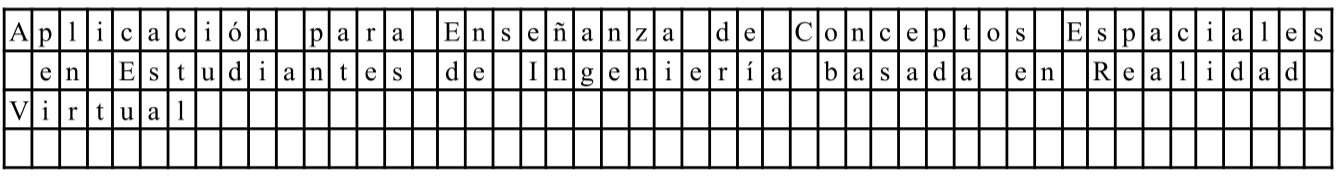
\includegraphics[width=\textwidth]{nombre-04-24.png}
\end{figure}

\subsection*{Datos del Estudiante:}
\begin{table}[h]
  \doublespacing
  \begin{tabularx}{\textwidth}{X c c c}
    \hline
    \textbf{Apellidos, Nombres} & \textbf{C.I.N.}    & \textbf{Teléfono}   & \textbf{e-mail}                    \\
    \hline
    \small{\estudiante}         & \small{28.031.941} & \small{04141919875} & \small{ajrosas.19@est.ucab.edu.ve} \\
    \hline
  \end{tabularx}
\end{table}

\subsection*{Datos del Tutor Académico:}

\begin{table}[h]
  \onehalfspacing
  \begin{tabularx}{\textwidth}{>{\hsize=.3\hsize}X X}
    Nombre                       & \academicTutor                                                                                     \\
    C.I.N.                       & 8.967.479                                                                                          \\
    Profesión                    & Ing. Computación                                                                                   \\
    Años Experiencia Profesional & 37 años                                                                                            \\
    Cargo Actual                 & Profesor                                                                                           \\
    E-mail                       & jlarez@ucab.edu.ve                                                                                 \\
    Teléfonos                    & 414-9875088 \tab Oficina: Escuela de Ingeniería Informática                                        \\
    \hline
    Años de Graduado             &
    37 años \tab[4cm] Tutor TG \hfill Sí \space\fbox{$\checkmark$} \hfill No \space\fbox{\phantom{a}}                                 \\
    \hline
    Profesor UCAB                & Sí \space\fbox{$\checkmark$} No \space\fbox{\phantom{a}} \tab[2cm] Escuela: Ingeniería Informática \\
  \end{tabularx}
\end{table}

\clearpage
